% !Mode:: "TeX:UTF-8"

\chapter{方法设计与实现}

\section{方法概述(Pipeline)}

该对象操纵交互系统的方法流程可以用一个有限状态机来表示,见图\ref{fig-3-1}。

\begin{figure}[b!]
    \centering
    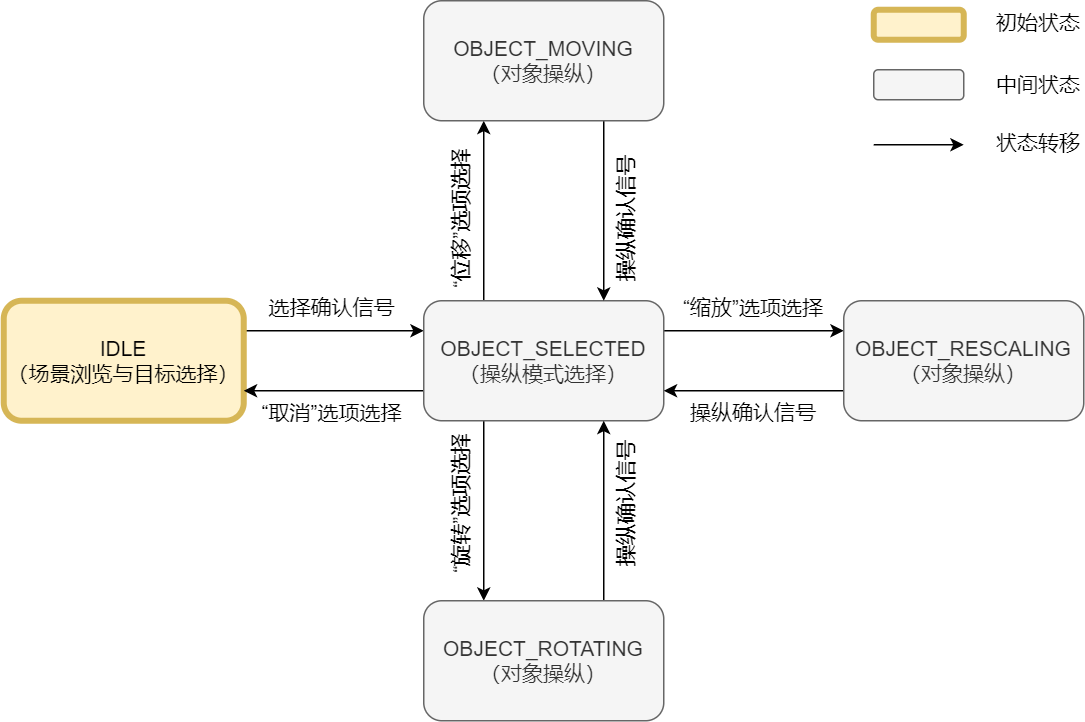
\includegraphics[width=.85\textwidth]{figure/system_state_machine.png}
    \caption{交互系统有限状态机}
    \label{fig-3-1}
\end{figure}

{\bf 场景浏览与目标选择}:对应状态IDLE。在进行目标选择时,用户先以通过头部向前射线指向目标操纵对象,之后以快速两次眨眼作为确认信号选择该对象,该选择和确认方法的优势由Yuan Yuan Qian团队在2017年作过探讨\upcite{yuanyuan2017}。接收到选择确认信号后,进入下一状态;

{\bf 操纵模式选择}:对应状态OBJECT\us SELECTED。生成一个“四叶草”模式选择菜单,用户可以通过凝视某一选项以进入对应的操纵模式,用户也可以通过凝视“返回”选项以退回到1(详见\autoref{Clover});

{\bf 对象操纵}:对应状态OBJECT\us MOVING、OBJECT\us ROTATING或OBJECT\us RESCALING。我们提出的操纵系统支持六自由度(6DOF)操纵。在不同的对象操纵模式下,用户可以对物体进行三自由度位移、二自由度旋转和一自由度缩放(详见\autoref{Manipulation});

{\bf 确认操纵结果}:对应状态转移条件“操纵确认信号”。通过快速两次眨眼作为确认信号以确认当前操纵状态,回到OBJECT\us SELECETD。

\section{场景浏览与目标选择}

该交互系统的浏览和选择方法不需要使用复杂的手柄或其他输入设备,使得用户能够更加自然地与虚拟环境进行交互。

\subsection{场景浏览}

在场景浏览时,该系统通过跟踪用户的头部向前(forward)射线控制场景中虚拟摄像头的移动,将其实时拍摄的场景画面即时反馈到用户的头戴式显示器中,以提供一个自然、直观的场景浏览体验。

其次,我们需要计算实时视点。视点的计算涉及到两个方面:视角和视位。视角是指用户在虚拟环境中的观察方向,通常由头部的旋转角度决定。视位是指用户在虚拟环境中的位置,通常由身体的移动或手柄的操作决定。为了实时地获取用户的视角和视位,需要使用一些传感器或追踪器,例如红外摄像头等。这些设备可以测量用户头部或身体的运动数据,并将其传输给计算机。根据用户的视角和视位,我们可以获取用户当前所期望观察、选中以及操作的物体。

在判断驻留点时,我们使用射线广播(ray-casting)的方法。射线广播是一种在虚拟现实中选择对象的常用技术;在我们的交互系统中,它利用用户的头部向前方向来发射一条射线,与场景中的对象进行碰撞检测,从而获取驻留点。射线广播的优点是简单、直观、高效、学习成本低并且不容易产生眩晕感和迷惑感。当驻留点在某个物体上时,该物体将被高亮,以消除对象选择时的歧义。同时,系统会在用户界面上与头部向前射线相交处生成一个瞄准点,帮助用户瞄准目标对象;该瞄准点仅会在IDLE状态下生成。当目标对象被瞄准后,用户可以通过快速两次眨眼来确认选择。

\subsection{目标选择}

在IDLE状态下,用户可以使用眼动确认信号来选择目标。该部分的主要挑战包括如何准确地捕捉并且解析用户的眼动数据以及如何提供合适的反馈和提示。

最为常见且自然的主动眼动信号有单眼眨眼和快速两次眨眼,因此我们将这两种眼动行为作为我们的最终眼动信号候选池。我们设计了一个前导实验(Pilot Study),目的是从这两种眼动信号中,确定一个最为高效并且带来最小使用压力的眼动确认信号,这将在之后的实验设计章节中作更细致的介绍。通过加权分析两种眼动行为的实验结果,我们最终确定使用快速两次眨眼来作为我们的目标选择以及确认信号。

在选择确认后,系统的状态转移到OBJECT\us SELECTED,并且会提供给用户一个基于听觉的声音反馈信号。这个反馈信号相对于视觉是异模态的,目的是提高交互系统的可靠性以及降低用户的迷惑感。

\section{“四叶草”模式选择菜单}\label{Clover}

\subsection{设计理念}

我们在交互系统设计阶段考虑到大多数实际的完整操纵流程往往不仅包含一个特定操纵模式的选择,还会包含多种操纵模式之间的切换。然而,当前的基于凝视和眼动的交互方法并没有考虑便捷的模式切换;在这些方法中,如果用户需要在一次操纵结束后切换到下一种操纵模式,则需要退回到最初态重新进行一遍从选择到操纵到流程,引入大量冗杂操纵和效率浪费。所以基于此考虑,我们设计了一个“四叶草”模式选择菜单。

我们希望“四叶草”模式选择菜单可以让用户简便地用凝视动作来选择进入或者切换到某种交互状态。

\subsection{菜单说明}

“四叶草”模式选择菜单在且仅在系统有限状态机的OBJECT\us SELECTED状态下生成在用户界面上,用户可以通过它来选择进入到某具体的交互模式:空间位移、空间旋转和空间等比例缩放,分别对应系统有限状态机中的OBJECT\us MOVING、OBJECT\us ROTATING和OBJECT\us RESCALING三个状态;用户也可以通过它来取消选中物体以回到IDLE态。这个过程可以在我们规定的系统有限状态机中体现\ref{fig-3-1}。

菜单在四个方向提供了四个的选项,分别为位移、旋转、缩放和取消;用户可以通过看向相应的方向来选择对应的选项。在规定每个方位具体对应哪个选项时,我们首先设置了一个问卷调查,发放给30个随机人员采样以获取用户根据推测对四个选项使用频率的排序;其次,我们参考Maxwell等人在2006年发表的结论(眼球水平运动的负担比垂直运动的负担小\upcite{2006Maxwell}),将问卷调查中显示最频繁使用的两种交互模式选项(位移、旋转)设置在左右两侧,将剩下的两种选项(等比缩放、取消)设置在上下两侧。

为了避免误触和“点石成金”的人机交互领域经典问题\upcite{2016Jacob},我们规定了一个选择确认时间;该时间默认为1秒,用户也可以根据自己的习惯调整时长。当用户选择时,界面上会显示一个选择确认进度盘,此时开始选择确认倒计时;进度盘会随着用户凝视射线持续指向选项而逐渐变满,用户可以在进度盘进度未满之前通过使视线复位来取消选择。当选择确认倒计时结束时,进度盘进度满,用户立即转移至凝视射线指向选项的对应状态。


\section{对象操纵}\label{Manipulation}

\begin{figure}[b!]
    \centering
    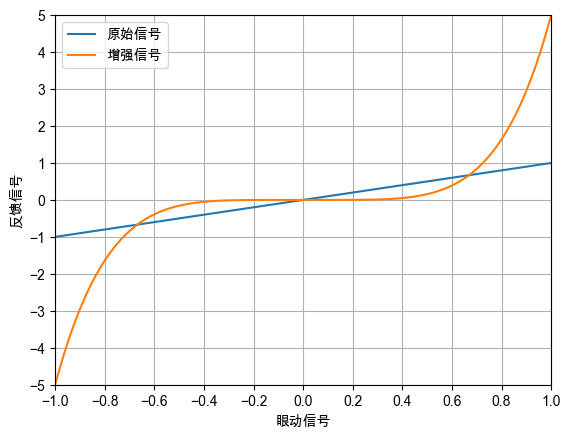
\includegraphics[width=.7\textwidth]{figure/augmented.png}
    \caption{信号增强函数}
    \label{fig-3-2}
\end{figure}

我们的交互系统支持完全6DOF的对象操纵,允许用户对目标对象进行空间位移、空间旋转、等比例缩放三种具体的操纵,分别对应系统有限状态机中的OBJECT\us TRANSLATING、OBJECT\us ROTATING和OBJECT\us RESCALING。

在每种对象操纵模式下,我们引入了一种特殊的信号增强函数:

\begin{equation}
	\label{formula-3-1}
	A(v) = 5v^{5}, -1 \le v \le 1
\end{equation}

让用户在小幅度动作时可以对对象进行微调,在大幅度动作时可以让对象作快速动作;其增强效果见图\ref{fig-3-2}。

为了减小操作负担和学习难度,我们都尽可能采用眼动进行主导的操纵,并且尽量不引入更多的操纵模态。为了便于接下来对具体操纵方法的阐释,我们在对象操纵空间中设置了一个三维直角坐标系,见图\ref{fig-3-3}。

\subsection{空间位移}

在空间位移时,对于X-Y平面的移动,对象跟随眼动向前射线在X-Y平面的投影距离作出相应的动作;假设眼动向前射线在X-Y平面的投影坐标为 $(x, y)$ ,对象在X轴向和Y轴向的移动为:

\begin{equation}
	\label{formula-3-2}
	\delta_x = 
    \left\{
    \begin{array}{l}
        0, \quad {\mbox{\boldmath $if$}}\ \left|x\right| < T \\ [0.2cm]
        x \cdot C,\quad {\mbox{\boldmath $default$}}
    \end{array}
    \right.
\end{equation}

\begin{equation}
	\label{formula-3-3}
	\delta_y = 
    \left\{
    \begin{array}{l}
        0, \quad {\mbox{\boldmath $if$}}\ \left|y\right| < T \\ [0.2cm]
        y \cdot C,\quad {\mbox{\boldmath $default$}}
    \end{array}
    \right.
\end{equation}

其中 $T$ 和 $C$ 分别是预先规定的阈值和比例系数。对于Z轴方向的移动,对象跟随头部以Z轴为旋转轴的角度-距离映射作出相应的动作;假设头动绕Z轴的旋转角度为 $\omega$ ,对象在Z轴方向的移动为:

\begin{equation}
	\label{formula-3-4}
	\delta_z = 
    \left\{
    \begin{array}{l}
        0, \quad {\mbox{\boldmath $if$}}\ \left|\omega\right| < T \\ [0.2cm]
        \sin{\omega} \cdot C,\quad {\mbox{\boldmath $default$}}
    \end{array}
    \right.
\end{equation}

其中 $T$ 和 $C$ 分别是预先规定的阈值和比例系数。

\subsection{空间定轴旋转}

在空间旋转时,对于以X轴的旋转,对象跟随眼动向前射线在Y轴的投影距离-角度映射作出相应的动作;对于以Y轴的旋转,对象跟随眼动向前射线在X轴的投影距离-角度映射作出相应的动作;假设眼动向前射线在X-Y平面的投影坐标为 $(x, y)$ ,对象在绕X轴向和Y轴向的旋转为:

\begin{equation}
	\label{formula-3-5}
	\delta_y = 
    \left\{
    \begin{array}{l}
        0, \quad {\mbox{\boldmath $if$}}\ \left|y\right| < T \\ [0.2cm]
        \frac{180}{\pi} \cdot x \cdot C,\quad {\mbox{\boldmath $default$}}
    \end{array}
    \right.
\end{equation}
 
\begin{equation}
	\label{formula-3-6}
	\delta_y = 
    \left\{
    \begin{array}{l}
        0, \quad {\mbox{\boldmath $if$}}\ \left|y\right| < T \\ [0.2cm]
        \frac{180}{\pi} \cdot y \cdot C,\quad {\mbox{\boldmath $default$}}
    \end{array}
    \right.
\end{equation}

其中 $T$ 和 $C$ 分别是预先规定的阈值和比例系数。

\begin{figure}[b!]
    \centering
    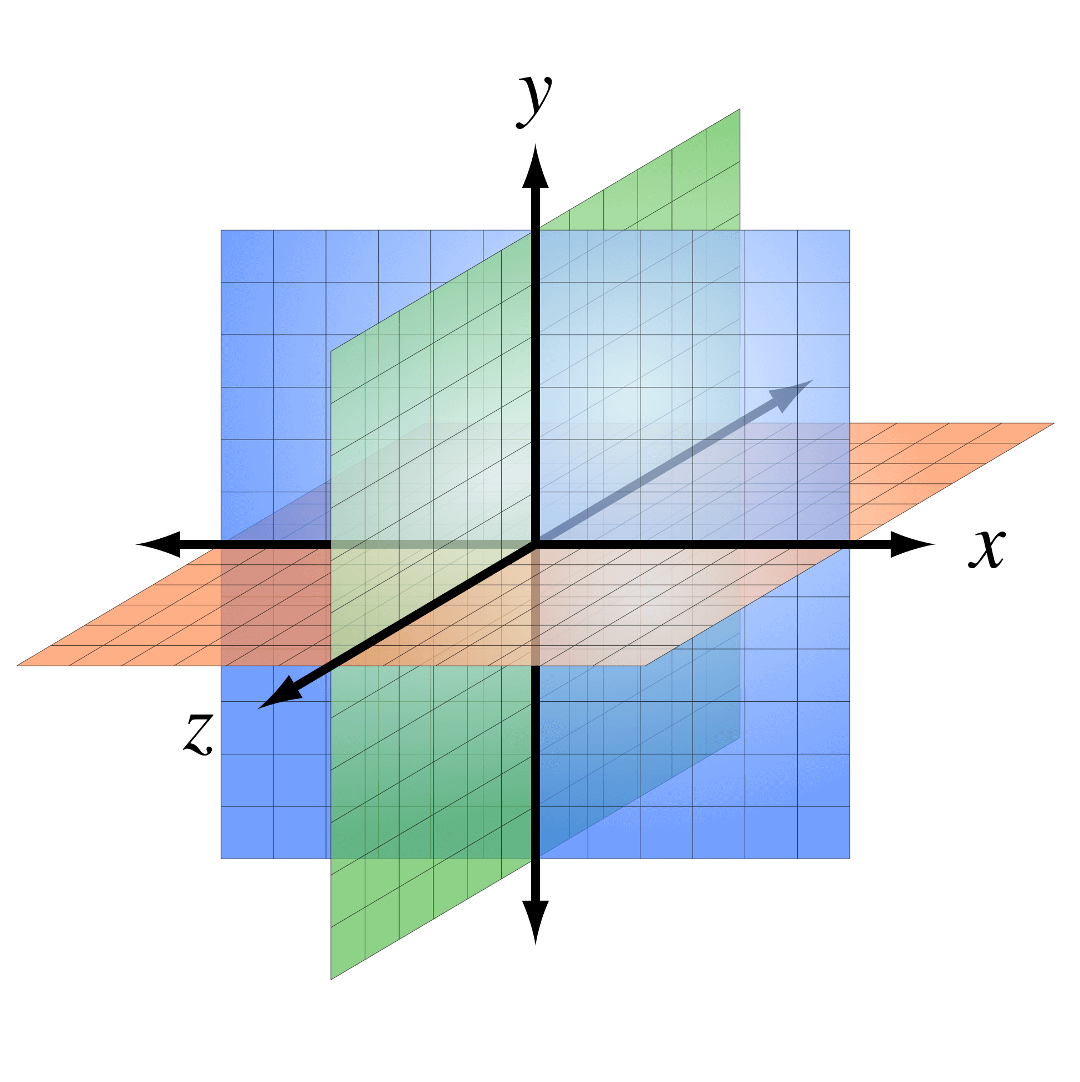
\includegraphics[width=.35\textwidth]{figure/coordinate.png}
    \caption{操纵空间坐标系}
    \label{fig-3-3}
\end{figure}

\subsection{空间等比例缩放}

在空间缩放时,对象跟随眼动向前射线在X轴的投影距离-缩放系数映射作出相应的动作;假设眼动向前射线在X轴的投影坐标为 $(x, 0)$ ,对象的缩放系数 $K$ 被计算为:

\begin{equation}
	\label{formula-3-7}
	K = 
    \left\{
    \begin{array}{l}
        0, \quad {\mbox{\boldmath $if$}}\ \left|y\right| < T\ {\mbox{\boldmath $or$}}\ x \le -1 \\ [0.3cm]
        2, \quad {\mbox{\boldmath $if$}}\ \frac{x}{C} \ge 1 \\ [0.2cm]
        1 + \frac{x}{C},\quad {\mbox{\boldmath $default$}}
    \end{array}
    \right.
\end{equation}

其中 $T$ 和 $C$ 分别是预先规定的阈值和比例系数;
对象的具体表现为 $Scale^\prime = Scale \cdot K$ 。

\section{信号处理}

\subsection{眼动信号滤波算法}

\begin{algorithm}[b!]
    \caption{针对该交互系统的眼动信号滤波算法}
	\begin{algorithmic}[1]
        \State SAMPLE $\leftarrow$ 5
 
        \State dataBuffer $\leftarrow$ EMPTY LIST of NUMBER
        \State currentBufferSize $\leftarrow$ dataBuffer.Count()

        \If {currentBufferSize $<$ SAMPLE}
        \For {i \textbf{in} Range(SAMPLE - currentBufferSize)}
            \State dataBuffer.Enqueue(GetData())
            \State Delay()
        \EndFor
        \Else
        \State dataBuffer.Dequeue()
        \State dataBuffer.Enqueue(GetData())
        \State Delay()
        \EndIf
        \State
        \State max $\leftarrow$ $-INF$
        \State min $\leftarrow$ $INF$
        
        \For {value \textbf{in} dataBuffer}
            \State max $\leftarrow$ value \textbf{if} value $>$ max \textbf{else} max
            \State min $\leftarrow$ value \textbf{if} value $<$ min \textbf{else} min
        \EndFor

        \State dataBuffer.RemoveFirst(max)
        \State dataBuffer.RemoveFirst(min)  

        \
        \State sum $\leftarrow$ 0
        \For {value \textbf{in} dataBuffer}
            \State sum $\leftarrow$ sum + value
        \EndFor
        \State \Return sum $/$ (SAMPLE -2 )
	\end{algorithmic} 
	\label{algorithm-3-1}
\end{algorithm} 

基于眼动的对象操纵方法的一大难点即眼动信号不稳定。其原因为:(1)眼部肌肉本能动作(如眨眼、跳视等)干扰频繁,引入大幅度的离群噪声信号,导致眼动信号解析难度大;(2)目前的眼动追踪设备信号无法做到采样率和分辨率的平衡,导致设备无法兼顾运算速度和捕捉精度,并且时常会出现随机的脉冲干扰。所以,我们为此提出了一种针对该交互系统的眼动信号滤波算法,让追踪设备可以在最低硬件消耗的基础上做到低噪声、平滑的眼动信号捕捉,见算法\ref{algorithm-3-1}。

该滤波算法基于中位值平均滤波法。中位值平均滤波算法是一种常用的数字信号处理方法,它结合了中位值滤波和算术平均滤波的优点,能有效地抑制脉冲噪声和周期性干扰,提高信号的平滑度和稳定性。中位值平均滤波算法的基本思想是:对于给定的一组采样数据,先去掉其中的最大值和最小值,然后对剩余的数据求算术平均值,作为该组数据的滤波输出。中位值平均滤波算法的优点有以下几个方面:(1)它能有效地消除由偶然出现的脉冲性干扰所引起的采样值偏差,保证了信号的真实性;(2)它对周期性干扰有良好的抑制作用,能够保留信号的基本特征;(3)它具有较高的平滑度,适用于高频振荡的系统;(4)该算法不需要排序,计算成本较低且反馈速度较快。

对于交互系统的某一时刻 $n$,我们对其前 $SAMPLE$ 帧接收的眼动信号采用中位值平均滤波算法,并将其返回值作为第 $n + 1$ 帧接收的眼动信号。

\subsection{平滑交互处理}

在目标选择以及操纵时,单纯依靠眼动或者头动的某一单一信号是不理想的;完全独立眼动和头动信号会使得交互流程不够自然,且很难实现微小幅度的交互动作,无法避免地会引入不必要的使用负担。因此,我们引入了一种头眼协同的信号处理函数,为交互过程引入更小的负担,使交互流程更加平滑。

平滑交互处理的核心思想即优化对凝视驻留点的计算方式。我们规定在 $t_0$ 时刻的眼动操纵注视停留 $OE$ 被计算为在时间段 $n$ 内的眼动向前射线和头动向前射线的配合角度偏移:

\begin{equation}
	\label{formula-3-5}
	OE_{t_0} = \frac{1}{n} \sum_{t=t_0-n}^{t_0} \left| \hat{eye_t} \cdot \hat{head_t} - \hat{eye_{t-1}} \cdot \hat{head_{t-1}} \right|
\end{equation}

其中,$\hat{eye}$ 是视线的单位向量,$\hat{head}$ 是头部注视的单位向量,$\cdot$ 是向量内积运算符。如果 $OE$ 小于某一阈值,则表示用户正在尝试注视。我们的一个先导实验表明,这个优化是必要的;它可以让交互流程更加平滑自然,引入更小的使用负担。